\documentclass[conference]{IEEEtran}
\IEEEoverridecommandlockouts
\usepackage{cite}
\usepackage{amsmath,amssymb,amsfonts}
\usepackage{algorithmic}
\usepackage{graphicx}
\usepackage{textcomp}
\usepackage{xcolor}
\usepackage{booktabs}
\usepackage{multirow}
\usepackage{balance}
\usepackage{url}

\def\BibTeX{{\rm B\kern-.05em{\sc i\kern-.025em b}\kern-.08em
    T\kern-.1667em\lower.7ex\hbox{E}\kern-.125emX}}

\graphicspath{{results_groq/}{results_surrogate/figures/}}

\begin{document}

% ── Title ───────────────────────────────────────────────────────────────────
\title{AI-Native Test Generation for Industrial Access Control:\\
       LLM-Guided XACML Request Synthesis
\thanks{Submitted to the 2nd International Conference on AI: AI-Native for
Universities and Industry (ICAI-FAI 2026), CMC University, Hanoi, Vietnam,
December~3, 2026.}
}

% ── Authors ─────────────────────────────────────────────────────────────────
\author{
\IEEEauthorblockN{1\textsuperscript{st} Cuong Nguyen Van}
\IEEEauthorblockA{\textit{Faculty of Information Systems} \\
\textit{School of Computing, Phenikaa University}\\
Hanoi, Vietnam \\
cuong.nguyenvan@phenikaa-uni.edu.vn}
\and
\IEEEauthorblockN{2\textsuperscript{nd} Duong Nguyen Minh}
\IEEEauthorblockA{\textit{Faculty of Information Systems} \\
\textit{School of Computing, Phenikaa University}\\
Hanoi, Vietnam \\
23010441@st.phenikaa-uni.edu.vn}
}

\maketitle

% ── Abstract ────────────────────────────────────────────────────────────────
\begin{abstract}
Attribute-Based Access Control (ABAC), standardized as XACML, is widely
adopted in Industrial Control Systems (ICS/OT) under IEC~62443 FR2 Use
Control. Authoring mistakes in XACML policies routinely produce
unauthorized-access or denial-of-service faults, yet testing these policies
at scale is both labor-intensive and methodologically challenging. Existing
mutation-testing and combinatorial-generation techniques are driven by policy
structure and do not model industrial attribute semantics. Large
Language Models (LLMs) offer domain-aware reasoning but lack formal coverage
guarantees and exhibit a documented permissiveness bias when generating
access-control artifacts. We propose AXIS-Gen, an AI-native test generation
framework combining structured, coverage-explicit LLM prompting with a
lightweight symbolic conflict-witness pass and a PDP-based mutation oracle.
On a representative ICS water-treatment-plant ABAC policy (6~rules, 51~mutants,
7~mutation operators, 5~seeds, request budget 40) evaluated with two real LLMs
(gpt-oss-120b and gpt-oss-20b via the Groq API), LLM-guided synthesis reaches
mean mutation scores of 77.6\% and 74.1\% (rule coverage 93.3\% and 90.0\%)
versus 53.3\% for random and 56.9\% for pairwise-combinatorial baselines,
i.e.\ $+$45.6\% and $+$39.0\% relative to random, and reaches 20 kills
2.1--2.2$\times$ faster. A deterministic surrogate that executes the same prompt
strategy without a language model reaches 94.1\%, i.e.\ the real models score
lower than this surrogate implementation of the strategy. In a paired ablation, both real
LLMs kill almost none of the combining-algorithm (RCM) mutants (0\% and 10\%);
a two-request symbolic conflict-witness pass kills the one killable RCM mutant
(the other is exhaustively shown to be equivalent), giving a small but
systematic gain of $+$0.8 to $+$2.0~pp.
\end{abstract}

\begin{IEEEkeywords}
AI-native testing, XACML, ABAC, LLM-guided test generation, mutation testing,
industrial control systems, IEC~62443
\end{IEEEkeywords}

% ============================================================
\section{Introduction}

\subsection{Context and Stakes}

ICS/OT environments are increasingly interconnected under Industry~4.0 and
cloud-assisted SCADA, and are exposed to cyberattacks.
IEC~62443 foundational requirement FR2 ``Use Control''~\cite{b10} concerns
enforcing authorized use of the system. Attribute-based access control (ABAC),
which has been proposed for ICS~\cite{b19,b20}, expresses such decisions in terms
of \textit{who} (subject role, clearance, location) may do \textit{what}
(action) on \textit{which resource} (type, zone, criticality) under
\textit{what conditions} (safety state, plant mode). A policy fault here is not
merely a data breach --- an over-permissive rule could let a vendor reconfigure
a safety PLC without authorization, and an over-restrictive rule could block a
cleared engineer from overriding a stuck interlock during a maintenance window,
both with potential physical consequences.

\subsection{The Testing Gap}

XACML's expressiveness makes policy authoring error-prone. We distinguish two
lines of prior work:

\textit{Stream A --- Mutation testing / coverage-based generation}
\cite{b1,b2,b3,b4,b5}: driven by policy structure (MC/DC, rule-pair coverage,
constraint-solver-based strong mutation), with no model of the industrial
attribute semantics that make certain combinations operationally meaningful or
adversarially dangerous.

\textit{Stream B --- LLM-guided test synthesis} \cite{b11,b12,b13,b14,b15}:
domain-aware, but lacking formal coverage guarantees; a 2025 study of
access-control policy synthesis \cite{b12} reports permissiveness issues:
generated policies were equivalent to the specification in 45.8\% of cases for
non-reasoning LLMs and 93.7\% for reasoning LLMs. To the best of our knowledge
(our literature search was not exhaustive), no prior work applies LLMs to XACML
request synthesis for ICS environments.

\textit{Gap:} We are not aware of an approach that combines LLM-level domain
reasoning with the coverage rigor that industrial ABAC policies call for. This
paper takes a first step in that direction.

\subsection{Contributions}

\begin{enumerate}
  \item \textbf{AXIS-Gen framework}: LLM synthesis + schema repair + symbolic
    conflict-witness pass + PDP oracle, producing XACML~3.0 request documents.
  \item \textbf{Empirical finding (RQ3)}: combining-algorithm faults are a
    systematic blind spot of sampling-only LLM approaches, observed with two
    real LLMs and a surrogate; root-cause analysis and a targeted fix via the
    symbolic pass, evaluated in a paired ablation.
  \item \textbf{Oracle design note}: under \texttt{deny-overrides}, a
    default-deny catch-all rule makes the top-level decision DENY for every
    request, so a decision-level oracle cannot distinguish mutants that leave
    that rule and the combining algorithm untouched; our reference policy
    therefore omits it (Section~III-D).
  \item \textbf{Reference implementation} (Python; fixed seeds forwarded to the
    LLM API; a few minutes per backend) with 5~figures and 4~tables per
    backend, evaluated with two real LLMs and an offline surrogate.
\end{enumerate}

% ============================================================
\section{Background and Related Work}

\subsection{XACML and ICS Security}

XACML~3.0~\cite{b9} provides a policy language (Rule/Policy/PolicySet), a
reference architecture (PEP/PDP/PAP/PIP), and three combining algorithms:
\texttt{deny-overrides}, \texttt{permit-overrides}, \texttt{first-applicable}.
Under IEC~62443 zones/conduits and security levels (SL1--SL4), ABAC/XACML
naturally expresses multi-axis access constraints. Production-grade open-source
PDPs include AuthzForce~\cite{b17} and WSO2 Balana~\cite{b18}.

\subsection{XACML Testing: State of the Art}

The approaches in Table~\ref{tab:related} are driven by policy structure;
to our knowledge none of them targets industrial attribute semantics.

\begin{table}[htbp]
\caption{XACML Testing Literature}
\label{tab:related}
\begin{center}
\begin{tabular}{|p{2.0cm}|p{2.5cm}|p{2.5cm}|}
\hline
\textbf{Work} & \textbf{Contribution} & \textbf{Limitation} \\
\hline
Martin \& Xie \cite{b1} & Fault model and mutation operators & Structure-driven \\
\hline
XACMUT \cite{b2} & XACML~2.0 mutant generator & Structure-driven \\
\hline
Strong mutation \cite{b3} & Tests derived with a constraint solver & Constraint encoding required \\
\hline
Coverage criteria \cite{b4} & MC/DC, rule-pair criteria & No industrial context \\
\hline
XACMET \cite{b5} & Request generation and model-based oracle & Structure-driven \\
\hline
\end{tabular}
\end{center}
\end{table}

\subsection{LLMs for Test Synthesis and Access Control}

Koziolek et al.~\cite{b11} prompt an LLM to synthesize test cases for PLC/DCS
control logic (function blocks of an open-source automation library) and
report high statement coverage for low-to-medium complexity programs; this is
a related use of LLMs for industrial test generation, but for control code
rather than access-control policies.
LLM permissiveness bias in policy synthesis~\cite{b12} motivates our design
decision to use LLMs only as request proposers, never as policy authors or
oracles. LACE~\cite{b13} combines LLM-based policy generation with formal validation
for IoT access control. Fuzz4All~\cite{b14} and ChatAFL~\cite{b15} use LLMs to
generate test inputs for language processors and for network-protocol
fuzzing, respectively.

\textit{Positioning:} We combine LLM-guided test synthesis with an XACML fault
model and a symbolic conflict-witness pass, targeting an industrial ABAC
policy.

% ============================================================
\section{Problem Formulation}

\subsection{Formal Policy Model}

A policy $P = \langle R_1, \ldots, R_n, \mathit{alg} \rangle$ where
$\mathit{alg} \in \{\texttt{deny-overrides}, \texttt{permit-overrides},
\texttt{first-applicable}\}$. Each rule $R_i = \langle \mathit{effect}_i,
\mathit{target}_i, \mathit{condition}_i \rangle$ where target and condition are
Boolean expressions over atomic predicates (\textit{category.attribute op
value}). The total attribute space $|D| = \prod_a |D_a| = 92{,}160$ for the
reference policy (9 attributes $\times$ finite domains).

\subsection{Reference Policy: ICS Water-Treatment Plant}

Table~\ref{tab:policy} shows the 6-rule reference policy under
\texttt{deny-overrides}. Rules R5 and R6 can fire on the same request (a vendor reading a historian
in the field zone during production), and so can R3 and R5 (a vendor
overriding a safety interlock in the field zone in the normal safety state);
by exhaustive enumeration of the 92{,}160-point attribute space these are the
only two of the 15 rule pairs that admit a common request.

\begin{table}[htbp]
\caption{Reference ICS Policy (deny-overrides, 6 rules)}
\label{tab:policy}
\begin{center}
\begin{tabular}{|c|c|p{2.2cm}|p{2.2cm}|}
\hline
\textbf{ID} & \textbf{Eff.} & \textbf{Description} & \textbf{Key Predicates} \\
\hline
R1 & PRM & Operators read HMI/PLC in control zones
   & role=op $\wedge$ action=read \\
\hline
R2 & PRM & Engineers read/write field--supv outside emergency
   & role=eng $\wedge$ mode$\neq$emerg \\
\hline
R3 & DNY & No override of safety interlock in normal state
   & action=ovrd $\wedge$ state=normal \\
\hline
R4 & PRM & Cleared on-site engineer overrides in maintenance
   & role=eng $\wedge$ state=maint $\wedge$ lvl$\geq$4 \\
\hline
R5 & DNY & Vendors denied field-zone access
   & role=vendor $\wedge$ zone=field \\
\hline
R6 & PRM & Vendors read historian in production \textit{[R5+R6 conflict]}
   & role=vendor $\wedge$ type=hist \\
\hline
\end{tabular}
\end{center}
\end{table}

\subsection{Fault Model: Seven Mutation Operators}

Adapting the fault models of~\cite{b1,b2,b3}, 7~operators produce 51~mutants
(Table~\ref{tab:mutants}).

\begin{table}[htbp]
\caption{Mutation Operators and Mutant Counts}
\label{tab:mutants}
\begin{center}
\begin{tabular}{|c|p{4.0cm}|c|}
\hline
\textbf{Op.} & \textbf{Seeded Fault} & \textbf{N} \\
\hline
RCM & Swap combining algorithm & 2 \\
\hline
CEM & Flip Permit$\leftrightarrow$Deny & 6 \\
\hline
CPM & Flip predicate operator & 22 \\
\hline
CVM & Shift numeric threshold $\pm$1 & 1 \\
\hline
TRM & Drop one Target predicate & 12 \\
\hline
LOM & AND$\to$OR in Condition & 2 \\
\hline
MRD & Delete entire rule & 6 \\
\hline
\multicolumn{2}{|c|}{\textbf{Total}} & \textbf{51} \\
\hline
\end{tabular}
\end{center}
\end{table}

\subsection{Oracle Design: The Default-Deny Masking Pitfall}

A default-deny catch-all rule under \texttt{deny-overrides} makes the
top-level decision DENY for every request (unless a rule evaluates to
Indeterminate). A decision-level oracle then cannot distinguish any mutant that
leaves the catch-all rule and the combining algorithm untouched. We therefore
deliberately omit this rule from the reference policy, so that NOT\_APPLICABLE
stays observable. We did not run an experiment with the catch-all rule; the
statement follows from the semantics of the combining algorithm.

% ============================================================
\section{AI-Native Test Generation Framework}

\subsection{Architecture Overview}

AXIS-Gen operates in five steps. \textit{Design principle:} the LLM is used
only as a domain-aware request proposer --- never as a policy author or oracle.
The PDP is the sole ground-truth authority, directly addressing the
permissiveness bias documented in~\cite{b12}.

\begin{enumerate}
  \item \textbf{Policy Ingestion \& NL Rendering}: the policy is defined in an
    internal representation (the prototype has no XACML parser); each rule
    carries a natural-language description, and the attribute domain table is
    rendered into the prompt.
  \item \textbf{LLM Prompt \& Generation}: structured prompt with 4 coverage
    objectives $\to$ JSON candidate requests.
  \item \textbf{Schema/Domain Repair}: normalize format drift (e.g.\ ``3''
    $\to$ 3), replace remaining out-of-domain values by random in-domain
    ones and count them; retry on empty/malformed output ($\leq$3 attempts).
  \item \textbf{Symbolic Conflict-Witness Pass}: brute-force enumeration of the
    finite attribute space (2.2~s measured on our machine) --- yields a witness
    for every rule pair that admits one.
  \item \textbf{PDP Oracle + Mutation Scoring}: ground-truth decisions; compute
    mutation score and coverage metrics.
\end{enumerate}

\subsection{Component 2: Structured LLM Prompt}

The system prompt prioritizes 4 objectives in explicit order, each mapped to a
known coverage criterion (Table~\ref{tab:prompt}).

\begin{table}[htbp]
\caption{LLM Prompt Objectives and Coverage Criterion Mappings}
\label{tab:prompt}
\begin{center}
\begin{tabular}{|c|p{1.8cm}|p{1.5cm}|p{1.3cm}|}
\hline
\textbf{P} & \textbf{Objective} & \textbf{Criterion} & \textbf{Targets} \\
\hline
1 & $\geq$1 request per rule & Rule Coverage \cite{b4} & MRD \\
\hline
2 & Flip each predicate, others fixed & MC/DC \cite{b4,b6} & CPM, CEM \\
\hline
3 & Values $n{-}1$, $n$, $n{+}1$ for thresholds & Boundary Value & CVM \\
\hline
4 & $\geq$1 request satisfying both targets of each rule-pair & Rule-Pair \cite{b4} & RCM \\
\hline
\end{tabular}
\end{center}
\end{table}

The prompt instructs the model to return only a JSON array whose keys are
\texttt{``category.attribute''} and whose values come from the declared finite
domains. The API does not enforce this schema, which is why the repair step
exists.

\subsection{Component 4: Symbolic Conflict-Witness Pass}

A \textit{conflict witness} for rule-pair $(R_i, R_j)$ is a request $r$ such
that both $R_i.\mathit{target}(r) \wedge R_i.\mathit{condition}(r)$ and
$R_j.\mathit{target}(r) \wedge R_j.\mathit{condition}(r)$ evaluate to true.
This is required to kill RCM mutants --- only when $\geq$2 rules fire
simultaneously does the combining algorithm determine the final decision.

\textit{Why prompting alone is insufficient for Objective~4:} finding a genuine
conflict witness is a constraint-satisfaction problem. Sampling merely hopes
to land in the right region --- consistent with the results in
Section~\ref{sec:rq3}. The prototype uses brute-force enumeration over
$|D|{=}92{,}160$ points; a production implementation could use an SMT or constraint
solver, as in~\cite{b3,b4}, for continuous or high-cardinality attributes.

% ============================================================
\section{Experimental Evaluation}

\subsection{Setup}

\begin{table}[htbp]
\caption{Experimental Configuration}
\label{tab:setup}
\begin{center}
\begin{tabular}{|p{2.8cm}|p{4.4cm}|}
\hline
\textbf{Parameter} & \textbf{Value} \\
\hline
Policy under test & ICS-WaterTreatment-ABAC-v1 (6 rules, deny-overrides) \\
\hline
Mutants & 51: RCM$\times$2, CEM$\times$6, CPM$\times$22, CVM$\times$1, TRM$\times$12, LOM$\times$2, MRD$\times$6 \\
\hline
Methods & Random, Pairwise-2way, LLM-Guided, LLM-Guided+Symbolic \\
\hline
Request budget & $\leq$40 per method (Pairwise stops once all pairs are covered: 30.4 on average) \\
\hline
Seeds & 5 (seed $\in \{1,\ldots,5\}$); one LLM call per seed \\
\hline
Kill threshold & 20/51 mutants \\
\hline
Attribute space & $|D|=92{,}160$ \\
\hline
LLM backends & gpt-oss-120b and gpt-oss-20b (Groq API; temperature 0.7, low reasoning effort, seed forwarded); deterministic surrogate as offline reference \\
\hline
Runtime & a few minutes per backend (dominated by API latency) \\
\hline
\end{tabular}
\end{center}
\end{table}

LLM-Guided+Symbolic reuses the \textit{same} LLM suite as LLM-Guided for each
seed and prepends the symbolic witnesses (2 requests), truncating the LLM
suite to keep the budget. LLM-Guided vs.\ LLM-Guided+Symbolic is therefore a
\textit{paired} ablation whose only difference is the symbolic pass.

\subsection{Metrics}

\begin{itemize}
  \item \textbf{Mutation score} $= |\text{killed}|/51$ --- primary effectiveness;
    a mutant is killed if at least one request receives a different PDP decision
    from the mutant than from the original policy.
  \item \textbf{Rule coverage} $=$ fraction of the 6 rules whose Target and
    Condition both hold for at least one request.
  \item \textbf{Req$\to$20-killed}: requests to kill 20/51 mutants (efficiency).
\end{itemize}

\subsection{Main Results (RQ1 and RQ2)}
\label{sec:rq12}

\begin{table}[htbp]
\caption{Main Results (5 seeds, budget $\leq$40, 51 mutants; mean $\pm$ std)}
\label{tab:results}
\begin{center}
\footnotesize
\setlength{\tabcolsep}{3pt}
\begin{tabular}{|l|l|c|c|c|c|}
\hline
\textbf{Method} & \textbf{Backend} & \textbf{\#Req} & \textbf{Mut.Score} & \textbf{RuleCov} & \textbf{Req$\to$20} \\
\hline
Random   & --- & 40.0 & 53.3\% $\pm$3.8 & 53.3\% & 16.0 \\
\hline
Pairwise & --- & 30.4 & 56.9\% $\pm$5.9 & 60.0\% & 13.2 \\
\hline
\multirow{3}{*}{LLM-Guided}
 & Surrogate    & 40.0 & 94.1\% $\pm$2.1 & 100\%  & 5.6 \\
  & gpt-oss-20b  & 29.4 & 74.1\% $\pm$6.2 & 90.0\% & 7.8 \\
  & gpt-oss-120b & 40.0 & 77.6\% $\pm$6.6 & 93.3\% & 7.2 \\
\hline
\multirow{3}{*}{LLM+Symbolic}
 & Surrogate    & 40.0 & 94.9\% $\pm$2.4 & 100\%  & 6.6 \\
  & gpt-oss-20b  & 31.2 & 75.7\% $\pm$6.3 & 90.0\% & 7.8 \\
  & gpt-oss-120b & 40.0 & \textbf{79.6\%} $\pm$6.6 & 93.3\% & 8.2 \\
\hline
\end{tabular}
\end{center}
\end{table}

\begin{figure}[htbp]
\centerline{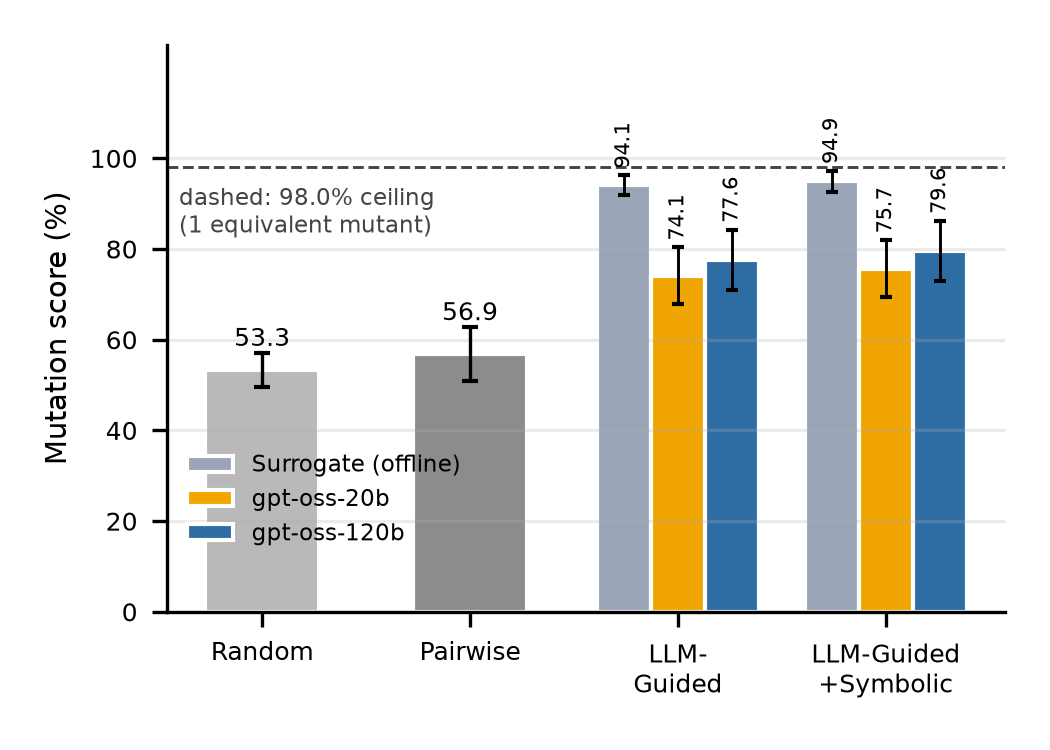
\includegraphics[width=\columnwidth]{fig_backends.png}}
\caption{Mean mutation score per method and backend (5 seeds, error bars
         $\pm$1 std). Real LLMs (orange, blue) clearly beat both baselines but
         stay below the offline surrogate (gray), which executes the same
         prompt strategy without a language model.}
\label{fig:mutation}
\end{figure}

\begin{figure}[htbp]
\centerline{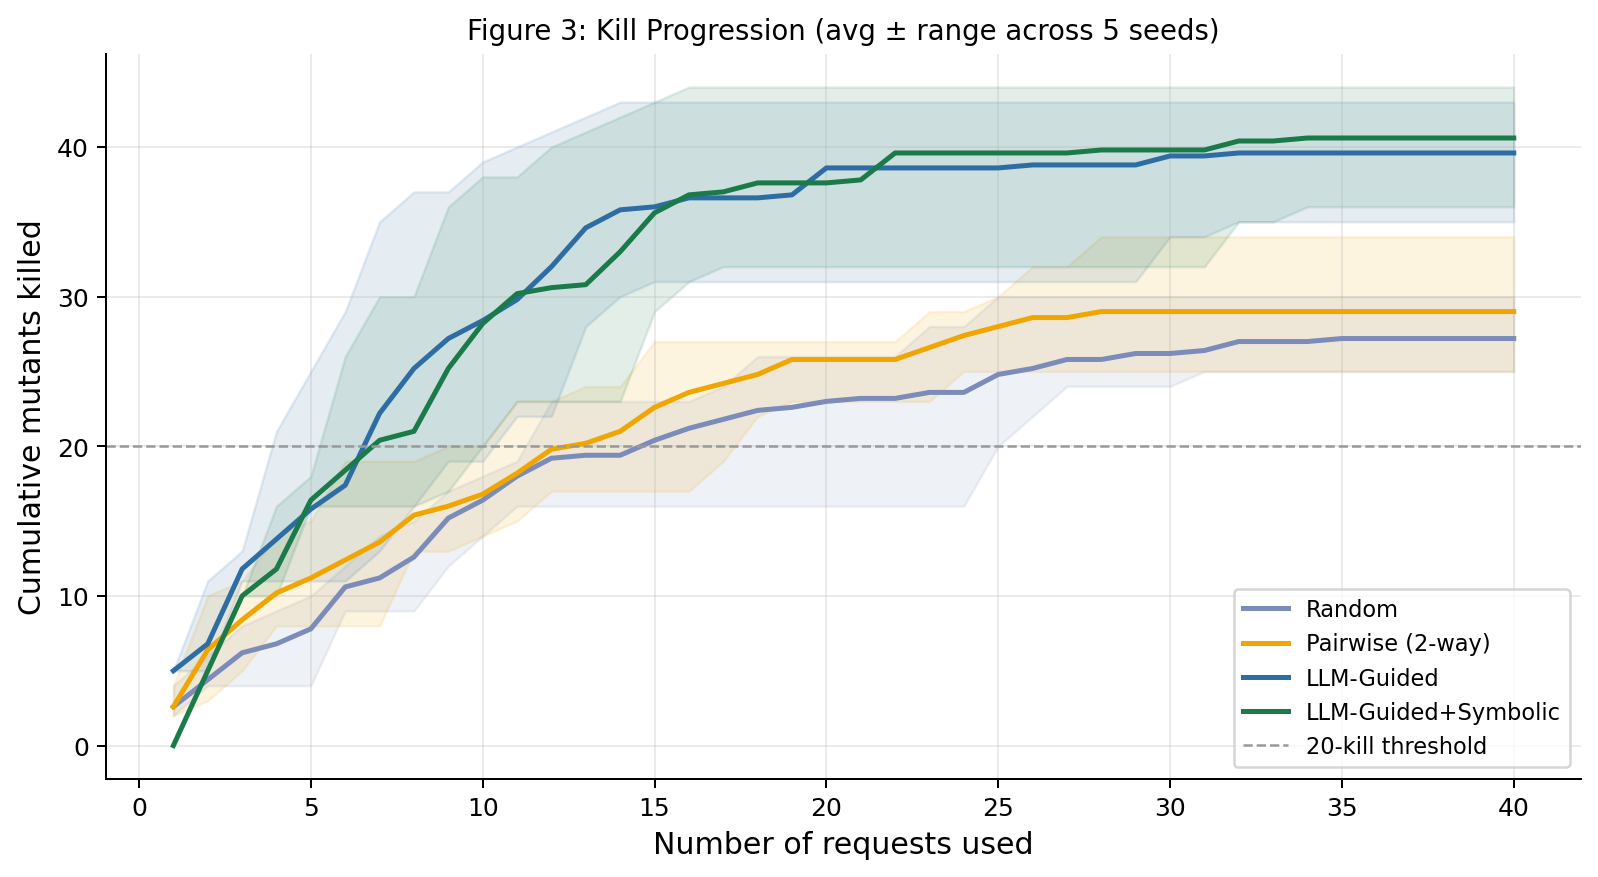
\includegraphics[width=\columnwidth]{fig_eff_120b.png}}
\caption{Kill progression (mean over 5 seeds, gpt-oss-120b). LLM-Guided reaches
         20 kills in 7.2 requests vs.\ 16.0 for Random (2.2$\times$).}
\label{fig:efficiency}
\end{figure}

\textbf{RQ1 (Effectiveness):} With real LLMs, LLM-Guided kills on average
39.6 (gpt-oss-120b) and 37.8 (gpt-oss-20b) of the 51 mutants versus 27.2 for
Random and 29.0 for Pairwise, a relative improvement of $+$45.6\% and
$+$39.0\% over Random and $+$36.6\% and $+$30.3\% over Pairwise. Rule coverage
is 93.3\% and 90.0\% versus 53.3\% (Random) and 60.0\% (Pairwise). The surrogate
(94.1\%, Table~\ref{tab:results}) scores higher than both real models; it is a
deterministic implementation of the prompt strategy and should not be read as
a proxy for a deployed model. The
improvement over the baselines is large relative to the seed-to-seed spread
($\pm$6.6 pp for gpt-oss-120b and $\pm$6.2 pp for gpt-oss-20b), but that spread
is also considerable. The reported values are the exact means of one 5-seed run
per model. gpt-oss-20b returned fewer requests than the budget in every seed
(13--39; 29.4 used on average), so its suites are smaller than those of the
other methods. The difference between the two LLMs (74.1\% vs.\ 77.6\%) is
within the seed-to-seed spread: we do not claim that the larger model is
better.

\textbf{RQ2 (Efficiency):} LLM-Guided reaches the 20-kill threshold in 7.2
(120b) and 7.8 (20b) requests vs.\ 16.0 for Random (2.2$\times$ and
2.1$\times$) and 13.2 for Pairwise (1.8$\times$ and 1.7$\times$). Pairwise consumes fewer
requests overall (30.4) because it terminates once all value pairs are covered.

\subsection{Combining-Algorithm Blind Spot (RQ3)}
\label{sec:rq3}

Fig.~\ref{fig:heatmap} breaks the kill fraction down by operator. Both real
LLMs kill at least 86\% of CEM, CPM and MRD mutants but only 60\%
(gpt-oss-120b) and 40\% (gpt-oss-20b) of CVM (boundary) mutants, and
essentially none of the RCM mutants: 0\% (gpt-oss-120b) and 10\% (gpt-oss-20b,
one seed). The offline surrogate also leaves both RCM mutants alive at a budget of 300
requests (49/51 killed); by design it does not implement prompt objective~4
(conflict witnesses), so this is expected and not independent evidence.

\begin{figure}[htbp]
\centerline{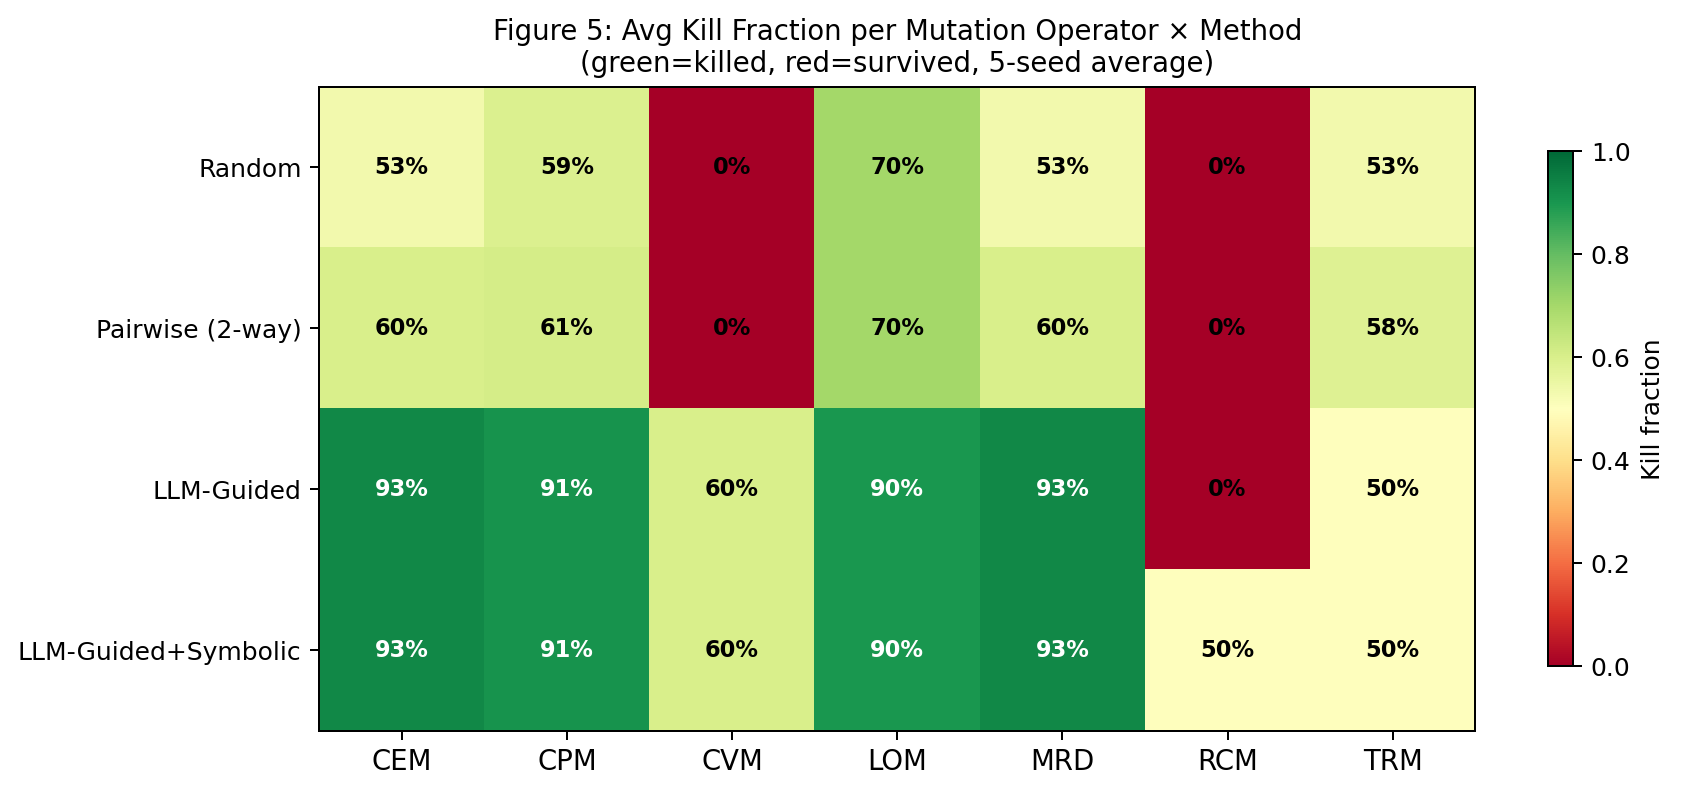
\includegraphics[width=\columnwidth]{fig_heat_120b.png}}
\caption{Kill fraction per mutation operator and method (gpt-oss-120b, 5-seed
         average). LLM-Guided kills 0\% of RCM mutants; the symbolic pass
         raises this to 50\%, the maximum attainable (see text). TRM is 50\% for both LLM-Guided and LLM-Guided+Symbolic.}
\label{fig:heatmap}
\end{figure}

\textbf{Likely cause:} killing an RCM mutant requires $\geq$2 rules to fire
simultaneously. The per-rule activation strategy (prompt objectives~1--3) does
not systematically construct multi-rule conflict witnesses even though
objective~4 asks for them --- finding one is a CSP, not a sampling problem.
The observation holds for both real models, which belong to the same model
family; it says nothing about other families.

\textbf{A second, open gap:} TRM (dropped Target predicate) mutants are killed
only about half of the time by every LLM variant (48--50\% across both models and both LLM methods). We
have not yet determined whether this is due to equivalent mutants or to a
genuine limitation of the prompt objectives.

\subsection{Hybrid Ablation (RQ4)}
\label{sec:rq4}

The symbolic pass adds two witness requests. Exhaustive evaluation of both RCM
mutants over all 92{,}160 inputs shows that \texttt{RCM\_permit-overrides}
differs from the original policy on 96 points, so it is killable, whereas
\texttt{RCM\_first-applicable} differs on \textit{none}: it is an
\textit{equivalent mutant}. The maximum attainable mutation score is
therefore 50/51 = 98.0\%, and the two witnesses kill the one killable RCM
mutant.

In the paired design the gain over LLM-Guided is $+$2.0~pp (gpt-oss-120b,
77.6\%$\to$79.6\%), $+$1.6~pp (gpt-oss-20b, 74.1\%$\to$75.7\%) and $+$0.8~pp
(surrogate, 94.1\%$\to$94.9\%). These gains are small (one mutant is
1/51 = 2.0~pp) and lie within the seed-to-seed spread, so with five seeds we
regard them as consistent with, but not proof of, a benefit; mechanistically,
however, the symbolic pass is the only component that reliably reaches RCM
mutants (the LLM-Guided suites of gpt-oss-20b killed an RCM mutant in one seed,
those of gpt-oss-120b in none).

\textit{Methodological note:} the ablation is deliberately paired. Two
witnesses can add at most $2/51 = 3.9$~pp (two mutants), so any larger
difference between the two methods would have to come from LLM sampling
variance rather than from the symbolic pass; letting the hybrid draw its own
independent LLM sample would therefore confound the comparison.

\textit{Trade-off:} Req$\to$20-killed increases by 1.0 for gpt-oss-120b
(7.2$\to$8.2) and for the surrogate (5.6$\to$6.6) and is unchanged for
gpt-oss-20b (7.8$\to$7.8), because the witnesses occupy the first two
positions of the hybrid suite. A production implementation could interleave
them by estimated fault likelihood.

\subsection{Evidence Scope and Research Integrity}

The LLM results come from two open-weight models (gpt-oss-120b, gpt-oss-20b)
served by the Groq API; no other provider was evaluated. The
\texttt{HeuristicSurrogateLLMClient} is a deterministic program executing the
same 4-objective prompt strategy \textit{without} a language model; its numbers
validate the \textit{strategy and the evaluation pipeline} and are reported
separately from, never as, LLM results. Domain validity of the real models was high: 4 of 1,800 attribute values
(gpt-oss-120b) and 2 of 1,323 (gpt-oss-20b) fell outside the declared domains
(0.2\% in both cases) and were replaced by random in-domain values by the
schema-repair step. The models did not always honor the requested count:
gpt-oss-120b returned 46--53 requests (truncated to the budget of 40), whereas
gpt-oss-20b returned 13--39, i.e.\ fewer than the 40 requested in all five
seeds (29.4 used on average, Table~\ref{tab:results}); no top-up call was made,
so the gpt-oss-20b suites are smaller than the gpt-oss-120b suites.

% ============================================================
\section{Threats to Validity}
\label{sec:threats}

\textbf{Construct validity:} Only two open-weight models from one family are
evaluated; results for frontier models (Claude, GPT, Gemini) may differ. The
surrogate validates the prompting strategy, not a deployed LLM. The prototype
PDP covers XACML~3.0 core but omits obligations/advice, multi-value bag
semantics, and XPath categories. A full study should use AuthzForce~\cite{b17}
or Balana~\cite{b18} as the production oracle.

\textbf{Internal validity:} Seeds are forwarded to the LLM API, but hosted
inference is not guaranteed to be bit-reproducible, and each backend was
run once (5 seeds), so run-to-run variability is not measured.
With five seeds and seed standard deviations of 6.6 (gpt-oss-120b) and 6.2
(gpt-oss-20b) pp for LLM-Guided and 6.6 and 6.3 pp for the hybrid, differences
of a few points (e.g.\ between the two LLMs, or between LLM-Guided and the
hybrid) are not statistically established; we report them descriptively and
make no significance claim.
Baseline spread: $\pm$3.8\,pp (Random), $\pm$5.9\,pp (Pairwise).

\textbf{External validity:} A single 6-rule policy cannot establish
generalization across policy sizes, combining algorithms, or attribute-domain
cardinalities. Study~3 (Section~\ref{sec:roadmap}) addresses this with a
benchmark corpus.

\textbf{LLM permissiveness bias (partially examined):} LLMs may
systematically under-sample deny-triggering combinations --- the worst failure
mode for a security test generator. As a first check, the share of requests that the PDP decides DENY is 14.5\%
for gpt-oss-120b (5.8 of 40) and 17.0\% for gpt-oss-20b (5.0 of 29.4), versus
8.5\% for Random. We therefore see no under-sampling of DENY outcomes relative
to random in this policy; PERMIT is the largest share (51.5\% and 43.5\%), and a
full audit remains part of Study~2.

% ============================================================
\section{Research Roadmap}
\label{sec:roadmap}

\begin{table}[htbp]
\caption{Priority Follow-Up Studies}
\label{tab:roadmap}
\begin{center}
\begin{tabular}{|c|p{2.0cm}|p{2.3cm}|p{1.0cm}|}
\hline
\textbf{\#} & \textbf{Question} & \textbf{Method} & \textbf{Priority} \\
\hline
1 & More real LLMs? & Done for gpt-oss-20b/120b; add Claude/GPT/Gemini & Critical \\
\hline
2 & Deny/safety bias? & Full audit beyond DENY share (Sec.~\ref{sec:threats}) & Critical \\
\hline
3 & Generalization? & Benchmark corpus + Z3 + AuthzForce & High \\
\hline
4 & Closed-loop? & Feed survivors as targeted kill prompts & Medium \\
\hline
\end{tabular}
\end{center}
\end{table}

% ============================================================
\section{Conclusion}

We presented AXIS-Gen, an AI-native test generation framework for industrial
XACML access-control policies. On a realistic 6-rule ICS policy with 51~mutants
and 7~mutation operators, LLM-guided generation with two real LLMs reaches
mean mutation scores of 77.6\% and 74.1\% at a budget of 40 requests
(gpt-oss-20b used 29.4 requests on average because it returned fewer than
requested), a $+$45.6\% and $+$39.0\% relative improvement in fault detection
over random generation, with 2.1--2.2$\times$ fewer requests needed to reach 20
kills. An
offline surrogate of the same strategy reaches 94.1\%, higher than both real
models. LLM-Guided almost entirely misses combining-algorithm (RCM) mutants; a two-request symbolic
conflict-witness pass kills the killable one (the other is provably
equivalent), a small but systematic gain of $+$0.8 to $+$2.0~pp that our five
seeds cannot confirm statistically.

Three observations from our experiments: (1)~LLM-guided generation with a
coverage-oriented prompt killed more mutants than random and pairwise
generation, with two mid-sized open-weight models on one policy;
(2)~combining-algorithm (RCM) mutants were reached reliably only by the
constraint-solving (enumeration) step and not by sampling; (3)~an ablation of
an LLM component should be paired (same LLM output with and without the
component), otherwise the effect is confounded with LLM sampling variance.

% ── Acknowledgment ──────────────────────────────────────────────────────────
\section*{Acknowledgment}

The authors thank the Faculty of Information Systems, School of Information
Technology, Phenikaa University for supporting this research.

% ── References ──────────────────────────────────────────────────────────────
\balance
\begin{thebibliography}{00}

\bibitem{b1}
E. Martin and T. Xie, ``A fault model and mutation testing of access control
policies,'' in \textit{Proc. WWW}, 2007, pp. 667--676.

\bibitem{b2}
A. Bertolino, S. Daoudagh, F. Lonetti, and E. Marchetti, ``XACMUT: XACML~2.0
mutants generator,'' in \textit{Proc. 8th Int. Workshop on Mutation Analysis},
2013, pp. 28--33.

\bibitem{b3}
D. Xu, R. Shrestha, and N. Shen, ``Automated strong mutation testing of XACML
policies,'' in \textit{Proc. ACM SACMAT}, 2020.

\bibitem{b4}
D. Xu, R. Shrestha, and N. Shen, ``Automated coverage-based testing of XACML
policies,'' in \textit{Proc. ACM SACMAT}, 2018, pp. 3--14.

\bibitem{b5}
S. Daoudagh, F. Lonetti, and E. Marchetti, ``XACMET: XACML testing \&
modeling,'' \textit{Software Quality Journal}, vol.~28, pp. 249--282, 2020.

\bibitem{b6}
F. Lonetti and E. Marchetti, ``On-line tracing of XACML-based policy coverage
criteria,'' \textit{IET Software}, 2018, arXiv:1809.02712.

\bibitem{b7}
A. Bertolino, Y. Le Traon, F. Lonetti, E. Marchetti, and T. Mouelhi,
``Coverage-based test cases selection for XACML policies,'' in \textit{Proc.
ICSTW}, 2014, pp. 12--21.

\bibitem{b8}
C. Caserio, F. Lonetti, and E. Marchetti, ``A formal validation approach for
XACML~3.0 access control policy,'' \textit{Sensors}, vol.~22, no.~8, art.~2984,
2022.

\bibitem{b9}
OASIS, ``eXtensible Access Control Markup Language (XACML) Version~3.0,''
OASIS Standard, Jan. 2013.

\bibitem{b10}
IEC, ``Industrial automation and control systems security,'' IEC~62443 series,
2018--2022.

\bibitem{b11}
H. Koziolek, V. Ashiwal, S. Bandyopadhyay, and C. K. R., ``Automated control
logic test case generation using large language models,'' arXiv:2405.01874,
2024.

\bibitem{b12}
A. Vatsa, B. Hall, and W. Eiers, ``Exploring large language models for access
control policy synthesis and summarization,'' arXiv:2510.20692, 2025.

\bibitem{b13}
Y. Cheng et al., ``Say what you mean: natural language access control with
large language models for Internet of Things,'' arXiv:2505.23835, 2025.

\bibitem{b14}
C. S. Xia, M. Paltenghi, J. Le Tian, M. Pradel, and L. Zhang, ``Fuzz4All:
universal fuzzing with large language models,'' in \textit{Proc. ICSE}, 2024.

\bibitem{b15}
R. Meng, M. Mirchev, M. B{\"o}hme, and A. Roychoudhury, ``Large language
model guided protocol fuzzing,'' in \textit{Proc. NDSS}, 2024.

\bibitem{b16}
NIST, ``Guide to attribute based access control (ABAC) definition and
considerations,'' SP~800-162, 2019.

\bibitem{b17}
AuthzForce Community Edition (OW2), ``ABAC/XACML PDP engine,''
\url{https://authzforce.ow2.org}, 2024.

\bibitem{b18}
WSO2, ``Balana --- open source XACML implementation,''
\url{https://github.com/wso2/balana}, 2023.

\bibitem{b19}
E. Yalcinkaya, A. Maffei, and M. Onori, ``Application of attribute based
access control model for industrial control systems,'' \textit{Int. J. Comput.
Netw. Inf. Secur. (IJCNIS)}, vol.~9, no.~2, pp. 12--21, 2017.

\bibitem{b20}
S. Gowdanakatte, M. Abdelgawad, and I. Ray, ``Security hardening of
industrial control systems through attribute based access control,'' in
\textit{ACSAC Industrial Control System Security (ICSS) Workshop}, 2023.

\end{thebibliography}

\end{document}
